% ================= 7. CONTROL ALGORITHMS & APPROACH =================
\section{Control Algorithms \& Approach}
\label{sec:control_algorithms}

This section derives the balancing controller from the linear models of
Section~\ref{sec:methodology}, states the controller as executable logic rather
than only as equations, describes the Simulink/Simscape environment used to
exercise that logic against both prototypes' CAD geometry before it runs on
hardware, and gives the onboard software architecture that carries it at
\qty{1}{\kilo\hertz} in flight. Detailed pseudocode, the fixed gains and
tuning parameters, the timing budget and the fault responses are collected in
Appendix~\ref{app:control_algorithms}.

\subsection{LQR Baseline Control}
\label{sec:control2d}

Linearising about the upright equilibrium $(\theta_b,\dot\theta_b,\dot\theta_w)=(0,0,0)$ gives
\begin{equation}
\dot x(t) = Ax(t) + Bu(t), \qquad x := (\theta_b,\dot\theta_b,\dot\theta_w),
\end{equation}
with $A, B$ built from the parameters in Table~\ref{tab:2d_vars}.
Zero-order-hold discretization at a rate set by the open-loop unstable pole,
with a safety margin, gives $x[k+1] = A_dx[k]+B_du[k]$. A discrete LQR gain
$K_d=(K_{d1},K_{d2},K_{d3})$ minimises
\begin{equation}
J(u) = \sum_k x^{\mathrm T}[k]Qx[k] + u^{\mathrm T}[k]Ru[k],
\end{equation}
giving $u[k]=-K_d(\hat\theta_b[k],\hat{\dot\theta}_b[k],\hat{\dot\theta}_w[k])$.
The same design generalises directly to the corner-balancing 9-state model of
Section~\ref{sec:3dmodel}: $K_d$ becomes a $3\times9$ gain matrix, using the
same discretization, cost function and offset filter below, with $Q, R$
weighting all three tilt axes, body rates and wheel speeds.

The tilt estimate $\hat\theta_b$ is obtained from a gyroscope and
accelerometer mounted at, or as close as mechanically feasible to, the pivot
point rather than at the plate's centre. This placement is necessary because
an accelerometer at radius $r$ from the pivot measures gravity plus the
tangential ($r\ddot\theta_b$) and centripetal ($r\dot\theta_b^2$) acceleration
components induced by the plate's rotation, which corrupt the naive estimate
$\tan^{-1}(-a_x/a_y)$ during fast motion (e.g., jump-up or aggressive
recovery); placing the sensor at $r\approx0$ makes both terms negligible.
Tilt is estimated with a complementary filter combining gyro integration
(drift-prone, unaffected by the terms above) with accelerometer inclination
(drift-free, but unreliable during shocks):
\begin{equation}
\hat\theta_b[k] = (1-\gamma)\big(\hat\theta_b[k-1] + \dot\theta_{b,\text{gyro}}[k]\,\Delta t\big) + \gamma\,\theta_{b,\text{accel}}[k],
\label{eq:complementary}
\end{equation}
where $\theta_{b,\text{accel}}[k] = \tan^{-1}(-a_x[k]/a_y[k])$ is the
instantaneous accelerometer-only estimate and $\gamma\in(0,1)$ is a small
weight favoring the gyro term between corrections.

A constant tilt-sensor offset $d$, including residual bias from imperfect
pivot placement or sensor misalignment, would otherwise appear as a nonzero
steady-state wheel speed rather than a corrected angle. A low-pass filter
state
\begin{equation}
x_f[k+1] = (1-\alpha)x_f[k] + \alpha\hat\theta_b[k]
\label{eq:offset_filter}
\end{equation}
is subtracted from the tilt feedback,
\begin{equation}
u[k] = -K_d(\hat\theta_b[k]-x_f[k],\, \hat{\dot\theta}_b[k],\, \hat{\dot\theta}_w[k]),
\end{equation}
so $d$ is absorbed by $x_f$ at steady state, requiring no separate calibration
stage. This fixed-gain design is the baseline balancing controller;
Table~\ref{tab:control2d_vars} summarizes the control variables.

\begin{table}[htbp]
\centering
\caption[Control-design variables]{Control-design variables (2D and corner-balancing 3D model).}
\label{tab:control2d_vars}
\begin{tabular}{ll}
\toprule
Symbol & Description \\
\midrule
$x$ & State vector \\
$A, B$ & Continuous-time state/input matrices (linearised model) \\
$A_d, B_d$ & Discrete-time (ZOH) counterparts of $A, B$ \\
$K_d$ & LQR feedback gain \\
$Q, R$ & LQR state/input weighting matrices \\
$J(u)$ & LQR cost function \\
$\hat\theta_b, \hat{\dot\theta}_b$ & Estimated tilt angle, rate (gyroscope/accelerometer) \\
$\hat{\dot\theta}_w$ & Estimated wheel rate (encoder) \\
$a_x, a_y$ & Raw accelerometer readings (tangential, radial axes) \\
$\theta_{b,\text{accel}}$ & Instantaneous accelerometer-only tilt estimate \\
$\dot\theta_{b,\text{gyro}}$ & Raw gyro rate measurement \\
$\gamma$ & Complementary-filter weight (accelerometer term) \\
$\Delta t$ & Control/estimation loop sample period \\
$x_f, \alpha$ & Offset-correction filter state, filter coefficient \\
$d$ & Constant tilt-sensor offset \\
$\theta_{\text{th}}$ & Tilt threshold, jump-up $\to$ balancing switch \\
$K_d^{(i)}$ & Scheduled gain at linearisation point $i$ (extension) \\
\bottomrule
\end{tabular}
\end{table}

\subsection{Gain Scheduling and Mode Transitions}
\label{sec:gain_scheduling}

The controller switches from the open-loop jump-up sequence to the LQR law
once $|\hat\theta_b| < \theta_{\text{th}}$, with hysteresis around
$\theta_{\text{th}}$ to prevent mode chattering. The baseline uses a single
fixed gain $K_d$ at the upright equilibrium. If recovery degrades near the
edges of the operating range, where the small-angle linearisation weakens,
gain scheduling will be added: additional gains $K_d^{(i)}$ computed at
several linearisation points, with the controller interpolating between them
based on $\hat\theta_b$, reusing the same discrete structure and offset
filter. The mode-transition logic gains a third mode for the 3D cube,
Edge-to-Corner jump-up, triggered once edge balancing is stable, followed by a
second threshold switch into the corner LQR once estimated orientation nears
corner-up; the full state machine is given in Table~\ref{tab:sw_modes}.

\subsection{Pure LQR Control Logic}
\label{sec:pure_lqr_logic}

Section~\ref{sec:control2d} derives $K_d$ offline, once, from the linear model.
What actually executes on the flight computer every control tick is the
sequence below, stated independent of how $K_d$ was computed so that the
running controller can be read, checked and re-implemented without
re-deriving the gain. Table~\ref{tab:control2d_vars} (2D) and its 3D
counterpart of Section~\ref{sec:3dmodel} define every symbol used; the fully
detailed pseudocode, including the supervisory state machine, is in
Appendix~\ref{app:control_algorithms}.

\begin{enumerate}
  \item \textbf{Sense.} Read raw gyro rate $\dot\theta_{b,\text{gyro}}$ and
        accelerometer $(a_x,a_y)$ from the IMU over SPI; read wheel angle(s)
        from the encoder(s) over the moteus CAN reply.
  \item \textbf{Estimate tilt.} Form the accelerometer-only estimate
        $\theta_{b,\text{accel}}[k] = \tan^{-1}(-a_x[k]/a_y[k])$ and fuse it
        with gyro integration through the complementary filter of
        Eq.~\eqref{eq:complementary} to obtain $\hat\theta_b[k]$.
  \item \textbf{Remove offset.} Update the low-pass offset state $x_f[k]$
        (Eq.~\eqref{eq:offset_filter}) and subtract it from $\hat\theta_b[k]$.
  \item \textbf{Assemble the state.} Build
        $\hat x[k] = (\hat\theta_b[k]-x_f[k],\ \hat{\dot\theta}_b[k],\ \hat{\dot\theta}_w[k])$
        in 2D, or the 9-vector $(\theta,\omega_b,\omega_w)$ of
        Section~\ref{sec:3dmodel} in 3D.
  \item \textbf{Check the mode.} If the supervisory state machine
        (Table~\ref{tab:sw_modes}) is not in a balancing mode, skip to
        step~8 and issue that mode's own open-loop command instead of
        $u[k]$ below.
  \item \textbf{Compute the command.} $u[k] = -K_d\,\hat x[k]$.
  \item \textbf{Saturate and manage momentum.} Clip $u[k]$ to the driver's
        continuous current rating (Appendix~\ref{app:bom}); if a wheel speed
        $\hat{\dot\theta}_w$ exceeds its desaturation threshold, add a small
        bias torque directed to bleed the stored momentum without
        materially perturbing $\hat\theta_b$.
  \item \textbf{Actuate.} Issue $u[k]$ (or the mode's open-loop command) as a
        CAN-FD torque request to each moteus driver.
  \item \textbf{Advance.} $k \leftarrow k+1$; repeat at the next
        \qty{1}{\kilo\hertz} tick (Section~\ref{sec:software_pipeline}).
\end{enumerate}

This is the loop exercised in simulation (Section~\ref{sec:sim_environment})
before it is exercised on hardware, and it is the loop whose worst-case
timing is bounded by construction in Section~\ref{sec:software_pipeline}.

\subsection{Simulation Environment: Simulink/Simscape Multibody}
\label{sec:sim_environment}

The control law of Sections~\ref{sec:control2d}--\ref{sec:pure_lqr_logic} is
validated in simulation before any closed-loop hardware run, on a plant built
from the same CAD geometry as the physical prototypes rather than from the
lumped-parameter equations alone --- so that the simulation catches geometry
effects (asymmetric mass distribution, off-axis clearances) the analytic model
cannot represent.

\paragraph{CAD-to-Simscape workflow.} Each CAD assembly --- the 1-DoF rig of
Section~\ref{sec:cad_2d} and the 3D cube of Section~\ref{sec:mechanical} --- is
exported as a STEP assembly and imported into Simscape Multibody, which
converts each part and mate into a rigid body and joint in a multibody tree.
The pivot bearing of the 1-DoF rig and the corner/edge contact features of the
3D cube are modelled as the corresponding revolute/point-contact joints, so
that the simulated degrees of freedom match Sections~\ref{sec:2dmodel}
and~\ref{sec:3dmodel} exactly rather than approximating them. Per-part mass and
inertia are taken directly from the CAD model, which is the same convention
that makes the mass roll-up of Section~\ref{sec:cad_method} auditable: the
simulation, the sizing, and the fabricated part all trace to one model.

\paragraph{Actuation and sensing blocks.} Each motor is represented as a
torque source at its joint, saturated and rate-limited to the envelope of
Section~\ref{sec:electrical}; the brake is a discrete event that zeroes the
relevant wheel-body relative velocity over the $\Delta t$ of
Equation~\eqref{eq:tau_b_from_dt}. Simulated IMU and encoder blocks apply
noise and bias models set from the sensors' characterised behaviour once
measured on hardware, so that the same estimator and control logic of
Section~\ref{sec:pure_lqr_logic} --- not a re-implementation of it --- runs
against simulated sensor data in a controller-in-the-loop configuration
before it runs against real sensors.

\paragraph{Test cases.} Three cases are run against the LQR baseline: recovery
from an initial tilt offset, which establishes the region of attraction;
rejection of an impulse disturbance applied at the body, which is the
simulated counterpart of the disturbance-recovery criterion the hardware is
later judged against; and behaviour under wheel-speed saturation, which
exercises the momentum-dumping step of Section~\ref{sec:pure_lqr_logic} and is
the case most likely to be missed by a purely linear analysis, since
saturation is precisely where the linear model ceases to describe the plant.
Each case is re-run with the plant parameters perturbed about their nominal
values, by a magnitude set once the identification tolerances of
Section~\ref{sec:paramid} are measured, so that the gains are shown not to be
knife-edge: a gain set that stabilises only the nominal plant is not a result,
because the nominal plant is not the one that will be built.

\paragraph{Direction of validation.} The measured parameters of
Section~\ref{sec:paramid} are substituted into the plant and the gains
re-derived before hardware balance is attempted; the simulation is validated
against the measured plant, never the reverse. A discrepancy between
simulated and measured closed-loop behaviour is treated as a finding about
the model.

No Simulink/Simscape model or CAD export exists yet at the time of writing;
this subsection states the workflow and the intended test cases, and is
populated with the model, the exported geometry and the resulting response
plots once built.

\subsection{System Integration}
\label{sec:integration}

\subsubsection{Onboard Software Pipeline}
\label{sec:software_pipeline}

The subsystems of Figure~\ref{fig:system_loop} are coordinated by a single
deterministic task on the Teensy, whose structure is given in
Figure~\ref{fig:software_pipeline}. Each \qty{1}{\milli\second} cycle executes
the same fixed sequence: sensor ingest reads the BMI270 over SPI and the moteus
replies over CAN; the MEKF propagates attitude on the gyro and corrects it
against the accelerometer while estimating gyro bias; the state vector
$x = [g_B, \omega, h]$ is assembled from the estimator output and the wheel
speeds; the LQR law of Section~\ref{sec:control2d} evaluates $u = -Kx$ with a
penalty on stored momentum $h$ to bleed off wheel saturation; and the resulting
commands leave as CAN torque requests to the drivers and a PWM signal to the
brake servos. Telemetry is tapped off the assembled state to SD and Wi-Fi outside
the control path, so logging cannot perturb loop timing.

The fixed ordering matters: with no dynamic allocation and no blocking calls, the
worst-case cycle time is bounded by construction rather than measured after the
fact, which is what makes the \qty{1}{\kilo\hertz} sample period of the discrete
LQR design a design guarantee rather than an average.

\begin{figure}[htbp]
\centering
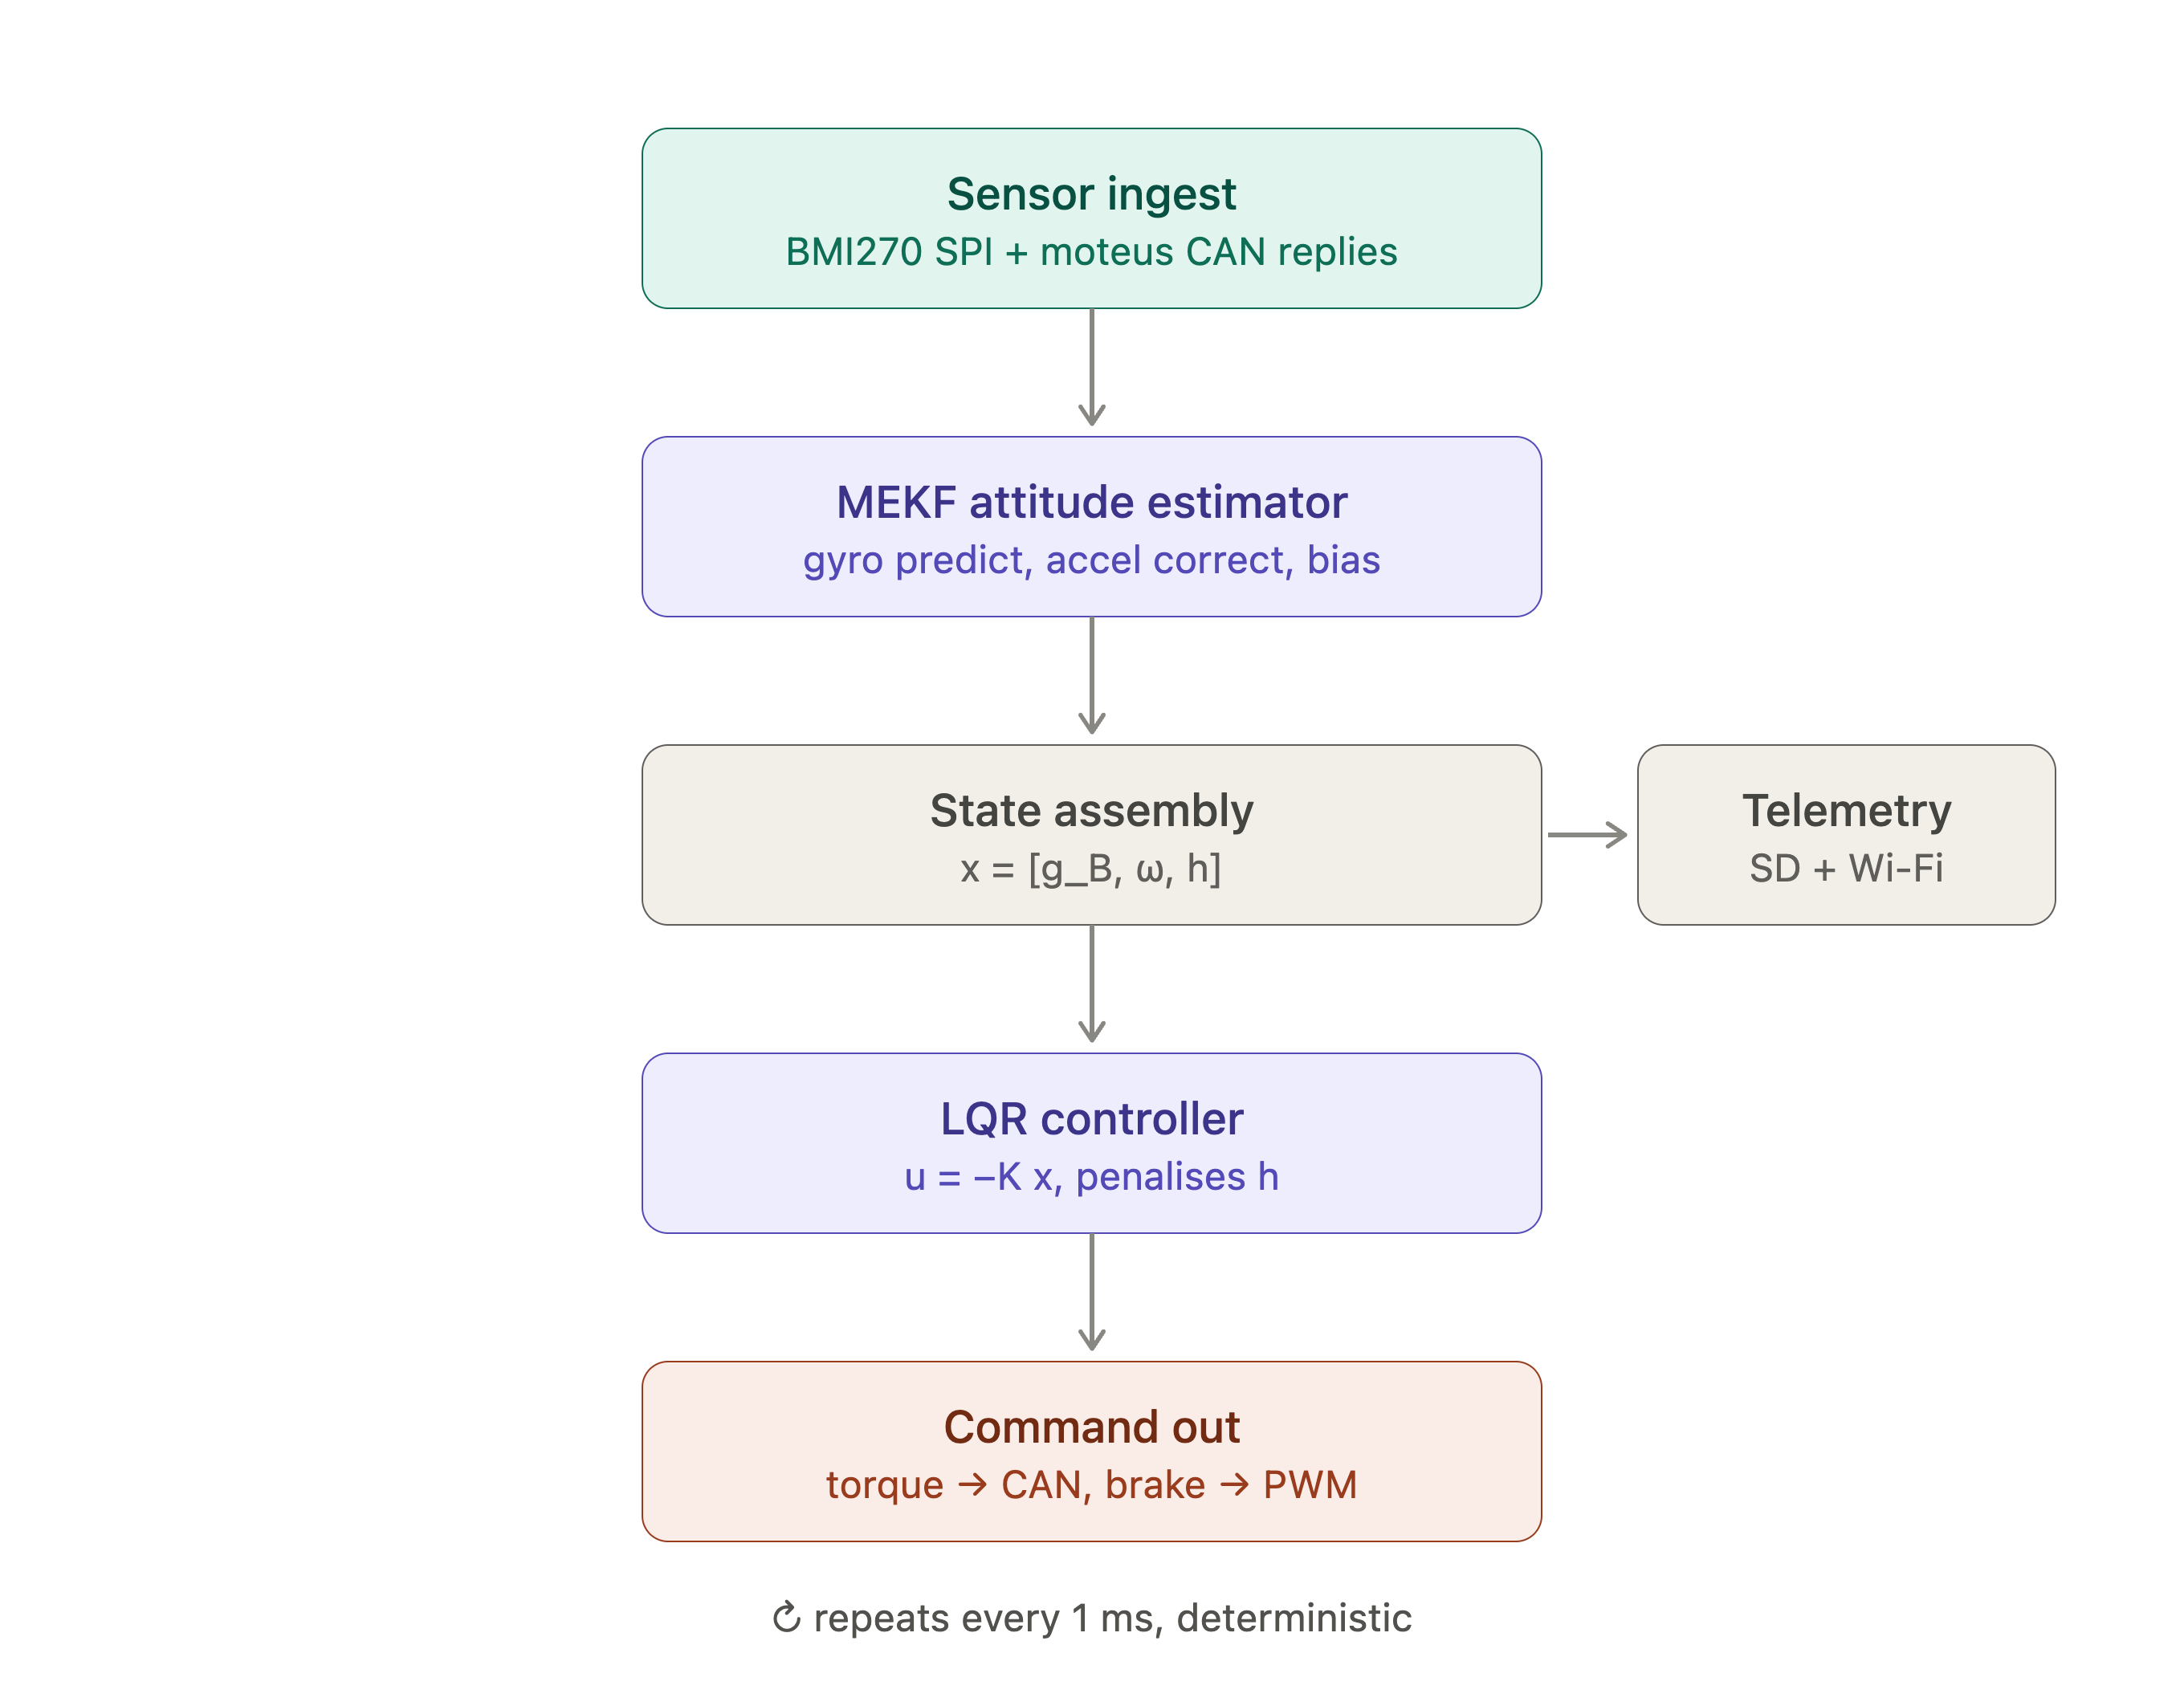
\includegraphics[width=0.78\textwidth]{images/teensy_software_pipeline.png}
\caption[Teensy 4.1 control-loop software pipeline]{Teensy 4.1 control-loop software pipeline. The estimator and controller
stages implement the design of Section~\ref{sec:control2d}; telemetry is a
side-branch off the control path.}
\label{fig:software_pipeline}
\end{figure}

\subsubsection{Control Software Architecture}
\label{sec:control_sw}

Sections~\ref{sec:control2d}--\ref{sec:pure_lqr_logic} derive the control law
and its executable logic; this subsection states how that law is realised as
software, which is a separate set of decisions. The implementation detail ---
the mode state machine, the estimator and controller in executable
pseudocode, the fixed gains and tuning parameters, the timing budget and the
fault responses --- is collected in Appendix~\ref{app:control_algorithms}, so
that a re-tuned gain does not require an edit to the design sections.

The software is organised in the four layers of
Table~\ref{tab:sw_layers}. The division is not stylistic: each layer has a
different failure mode and a different verification method, and the interfaces
between them are what allow the controller validated in simulation
(Section~\ref{sec:sim_environment}) to be the same code that runs on the cube.

\begin{table}[htbp]
\centering
\caption[Control software layers]{Control software layers. Each is verified by a different method, which
is why the boundaries are held.}
\label{tab:sw_layers}
\small
\begin{tabular}{L{2.8cm} L{5.4cm} L{5.6cm}}
\toprule
Layer & Responsibility & Verified by \\
\midrule
Hardware abstraction & Sensor and driver I/O, timing, bus transactions & Bench read-back; loop-timing measurement \\
Estimation           & Attitude and rate estimate from IMU and encoders (Sec.~\ref{sec:control2d}) & Static and dynamic bench tests against a known reference \\
Control              & State feedback, momentum management, saturation handling & Simulation on the identified model, then hardware \\
Supervision          & Mode transitions, arming, watchdog and fault response & Fault-injection tests on the rig \\
\bottomrule
\end{tabular}
\end{table}

\paragraph{Operating modes.} The supervisory layer sequences the modes of
Table~\ref{tab:sw_modes}, with hysteresis on every threshold to prevent
chattering at a boundary, and with a disarm transition available from every
mode. The modes are specified as a state machine because the critical
transitions are the descending ones: a fall detected during corner balance must
reach a safe state with the wheels commanded down, not merely switch to a
different gain.

\begin{table}[htbp]
\centering
\caption[Operating modes and transitions]{Operating modes and transitions. Every mode has a disarm exit.}
\label{tab:sw_modes}
\small
\begin{tabular}{L{2.6cm} L{5.2cm} L{6.0cm}}
\toprule
Mode & Behaviour & Exit condition \\
\midrule
Idle / disarmed & Drivers de-energised; sensors and telemetry live & Explicit arm command \\
Wheel spin-up   & Open-loop speed ramp to the jump-up momentum target & Target wheel speed reached \\
Jump-up         & Brake actuation and momentum transfer (Sec.~\ref{sec:jumpup}) & Tilt inside the balancing capture band \\
Edge balance    & Single-axis state feedback (Sec.~\ref{sec:control2d}) & Corner-transition command, or fall detected \\
Corner balance  & Three-axis state feedback (Sec.~\ref{sec:3dmodel}) & Slew command, or fall detected \\
Slew / rotation & Reference tracking between equilibria & Reference reached; revert to balance \\
Fault / safe    & Wheels commanded down, drivers disarmed & Manual reset \\
\bottomrule
\end{tabular}
\end{table}

\paragraph{Real-time guarantees.} The loop-rate claim of
Section~\ref{sec:control2d} is a design guarantee only if the worst-case cycle
is bounded by construction, which is why the pipeline of
Figure~\ref{fig:software_pipeline} uses a fixed stage ordering with no dynamic
allocation and no blocking calls, and why telemetry is a side-branch rather than
a stage.

\paragraph{Fault handling.} The failure cases the software must survive are
sensor dropout, bus error, wheel saturation and loss of the balancing
equilibrium. The first three have defined responses that keep the machine
controlled; the fourth is a controlled shutdown rather than a recovery attempt,
since a cube that has left its capture region cannot be recovered by the
linear law and continued actuation only adds energy to the fall.
